\section{Design Overview}
\label{sec:overview}


\begin{figure}[tb]
\centering
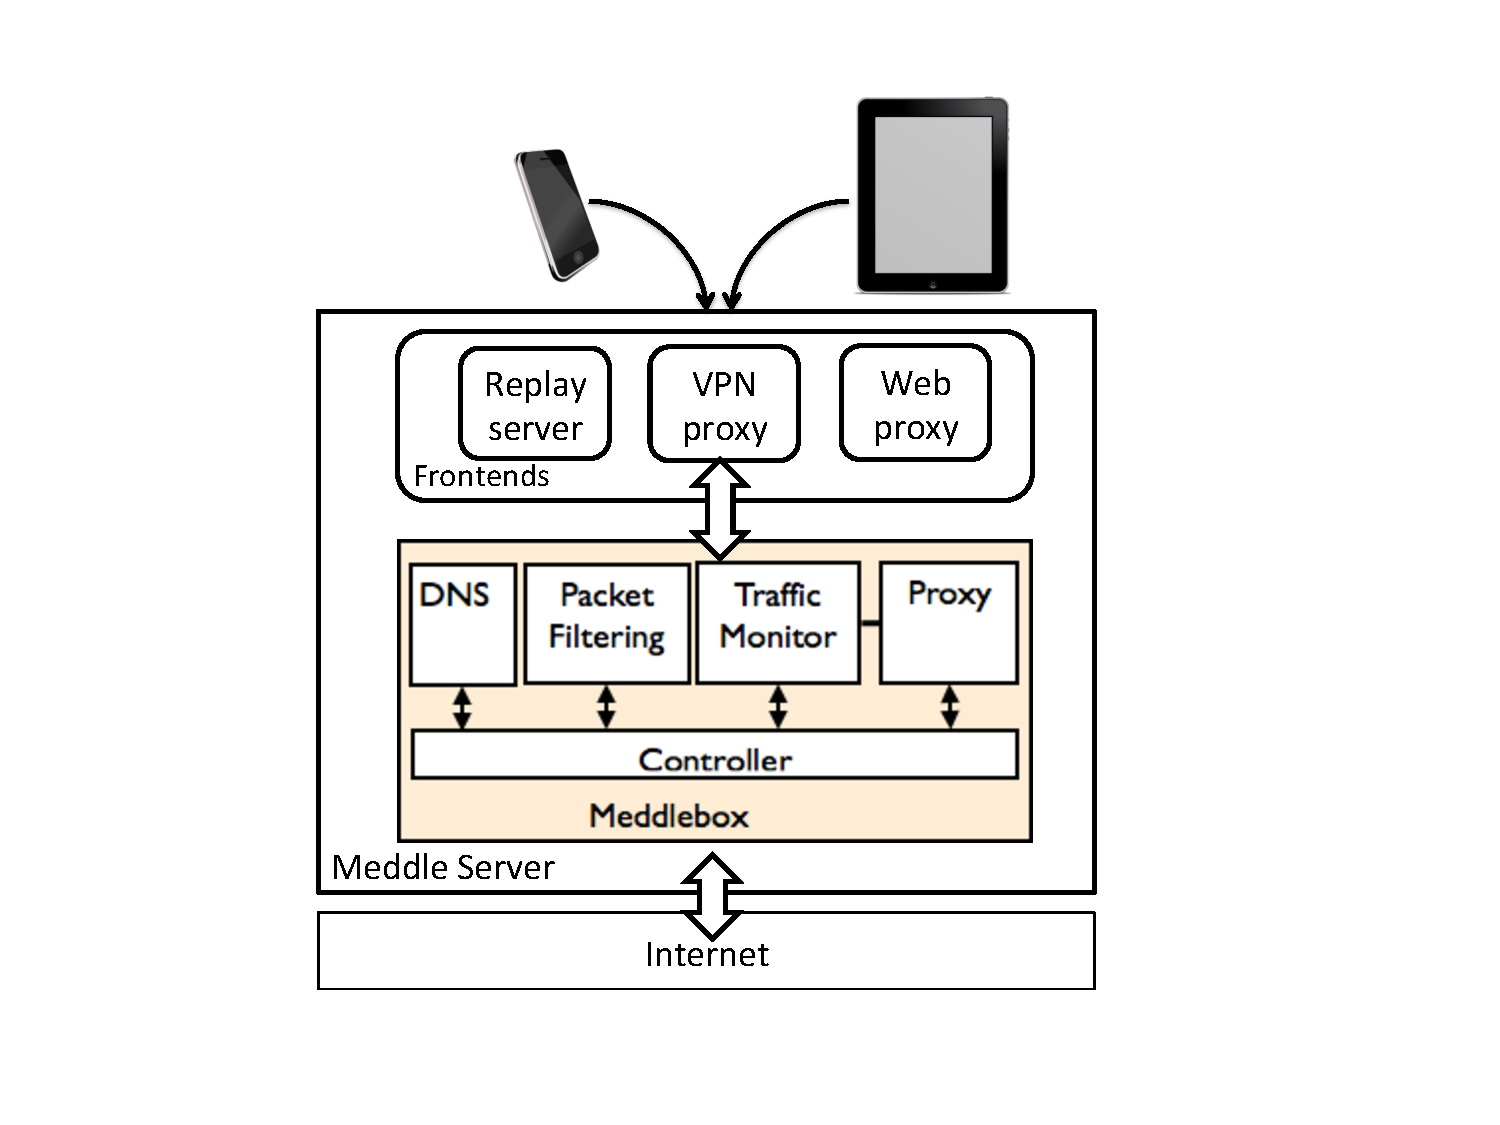
\includegraphics[width=0.8\columnwidth]{figures/meddle-diagram.pdf}
\caption{Architecture for \meddle. Mobile devices (top) communicate with 
a \meddle frontend (VPN proxy, Web proxy and/or 
traffic replay server). VPN proxy traffic is forwarded to a \meddlebox, which provides 
software middlebox services that measure and/or interpose on network flows before 
relaying the traffic to the Internet.  }
\vspace{\postfigspace}
\label{fig:architecture}
\end{figure}

\meddle's design consists of three core components: VPN tunnels from client to meddle server; packet capture and monitoring tools at the server; and server-side {\it meddlebox} services which may interpose on user traffic \eg{}, to filter unwanted traffic or apply performance enhancements such as image compression. This architecture is illustrated in Figure~\ref{fig:architecture}. These three simple components allow us to achieve our key goals:

\noindent\textbf{Visibility}. We aim to capture all of a mobile-device's Internet traffic,
allowing us to characterize network flows and interpose on them using software middleboxes.
To achieve this, we need a solution that works continuously, regardless of the mobile OS, network/access 
technology, or apps installed. 
Almost all modern mobile devices support VPN connections which are always-on or available on-demand. 
VPN connections allow us to capture {\it all} traffic generated by or sent to the device; importantly, users may enable or disable this at any time with a single switch.
  
\noindent\textbf{Control}. Another important goal is to facilitate research into new middlebox approaches 
for interposing on mobile Internet traffic. The system must support the ability to deploy and distribute large numbers 
of middlebox services quickly, easily and at scale~\cite{sherry:middleboxes} without 
the need to deploy hardware in homes~\cite{bismark} or ISPs~\cite{wang:middleboxes}. 
It should present a simple API for researchers and developers to block, shape, inject or otherwise 
modify network flows. It should also support applications that operate on collections of flows over 
time and across users (\eg Web caching/prefetching, malware detection/blocking and ISP characterization). 
As we will discuss in the section~\ref{sec:server}, the Meddle server architecture allows for easy addition or removal of new middlebox services.
Researchers can readily experiment with services for a large number of users without interacting with service providers; users have the option to opt-in to any collection of services they are interested in via a web interface. 


\noindent\textbf{Deployability}. To improve the representativeness of studies using \meddle, we want to 
recruit average (\ie, non-technical) users to participate in our system. To support this, we need a system 
that has incentives for users, a low barrier to adoption, is easy to deploy and that scales gracefully. 
The meddle approach has a low barrier to adoption in that it requires the installation of a single piece of software by users -- they do not need to `jailbreak' their operating systems, nor do they need to contract with a specific service provider. 
Both Android and iOS support the meddle software, and any mobile device with a data connection can connect to a meddle server.
The meddle approach has strong user incentives by way of the network services meddle provides.
In later sections (\S\ref{sec:applications}), we present user services that allow users to control their privacy, detect traffic manipulation by their provider, and improve their network performance.
All a user need to is install the meddle software and opt-in to service via a simple web interface.

In the following sections, we discuss the \meddle architecture in depth: first from the user perspective (\S\ref{sec:user}), then from the server-side and researcher's perspective (\S\ref{sec:server}). We then briefly evaluate some of \meddle's overheads and system performance.

\section{User Side Implementation}
\label{sec:user}
A user's interaction with \meddle consists of two primary steps: signing up for \meddle and enabling the VPN, followed by interacting with network services applied to their traffic.


\subsection{Setting up Meddle}
\meddle leverages the fact that the vast majority of mobile devices provide native VPN support, a feature typically provided to satisfy enterprise clients. We currently support VPN tunnels on iOS and Android; we anticipate being able to support the next version of Windows Phone that includes a native VPN implementation.

To use \meddle, a user signs up at our website (\url{www.meddle.mobi}) and receives an invitation email with account information and installation instructions. In our user studies, we found that users were easily capable of following our step-by-step instructions to enable \meddle; thus we believe that \meddle has reasonably low barriers to adoption. 

\noindent\textbf{iPhone support.} 
Once a user has their account information, they follow the standard operating system interface for enabling a VPN, the same interface as an employee enabling a VPN for their company. Once they enable the VPN, all of a user's traffic is directed to the meddle server; this can easily be disabled by simply turning off the VPN.

All iOS devices (version 3.0 and above) support \textit{VPN On-Demand}, which forces traffic for a specified set of domains to use VPN tunnels; we use a wildcarded list of domains to ensure that {\it all} domains a user contacts go through the VPN. 
%This feature is originally intended to allow enterprises to ensure their employees' devices always establish a VPN connection before contacting a specified set of domains. 
%To ensure all possible destinations match this list, we exploit the fact that iOS uses suffix matching to determine which connections should be tunneled; accordingly, we specified the domain list as the set of alphanumeric characters (a-z, 0-9, one character per domain). 
To setup this configuration, users need to install a single file, a step that is performed once during setup. 

\noindent\textbf{Android support.} 
Once a user has received their account information, they install an official Meddle app which wraps the StrongSwan VPN client~\cite{strongswanclient}. 
Like the iPhone process, the user enters the credentials (only five fields) they received in their email; once again, disabling \meddle requires only the click of a button within the \meddle app.

As of Android 4.2, Android supports ``always on'' VPN connections that ensure all traffic is always tunneled;
For Android version 4.0 and above there is an app API that allows apps to manage VPN tunnels; our wrapper of the StrongSwan client ensures re-establishment of VPN tunnels on network state changes (\eg, when a device switches from cellular to \wifi).
\meddle thus supports devices running Android version 4.0 and above.

\subsection{Meddle Apps}

Once a user has installed meddle, they benefit from numerous network services. Most are passive -- users do not see them directly, but, \eg{} can rest assured that their traffic is more secure. Others are more active -- for example, we provide a user interface to allow users to observe directly what ad and analytic servers their phone is contacting and block unwanted traffic. Together, these applications provide users users with good incentives to install and use \meddle.

%\begin{packeditemize}
\noindent \emph{Improved security.} By securely tunneling all of a mobile device's traffic, users 
are less vulnerable to data leakage (\eg via open WiFi hotspots). 

\noindent \emph{Device-wide content filters.} We use \meddle to block content that users do 
not wish to access -- for all apps running on a device. The most popular instance of this is 
device-wide ad blocking.

\noindent \emph{Privacy revelations~\cite{wetherall:revelations}.} The \emph{ReCon} tool (\S\ref{subsec:recon}) allows users to see how they are being 
tracked by ad and analytic servers, and allows them to create per-connection block lists.  

\noindent \emph{ISP transparency.} We provide services that allow users to identify cases where 
ISPs are modifying HTTP content in flight, and when they provide differentiated service to 
traffic crossing their networks (\S\ref{sec:isp-behavior}).

\noindent \emph{Malware detection.} \meddle uses network signatures to identify malware, block it from 
communicating and prevent future downloads onto other \meddle-enabled devices (\S\ref{sec:malware}).  
%\end{packeditemize}



\section{Meddle Server Implementation}
\label{sec:server}

As we described in \S\ref{sec:overview} and illustrated in Figure~\ref{fig:architecture}, \meddle has three key architectural components: VPN connections to each client (\S\ref{subsec:vpn}), traffic monitoring and logging tools (\S\ref{subsec:monitoring}), and {\it meddlebox} network services (\S\ref{subsec:meddlebox}). We now discuss the implementation of each of these components within the \meddle server. 

\subsection{VPN Connections}
\label{subsec:vpn}
\meddle uses the free and open-source Strongswan~\cite{strongswan} to manage the VPN tunnels 
on its servers. 

\subsection{Packet Capture and Monitoring}
\label{subsec:monitoring}
When traffic arrives at the server, we use \emph{tcpdump} and \emph{bro} to record 
traffic. We use two IRB-approved measurement approaches. One approach captures full packets, 
and requires subjects to be interviewed and provide written informed consent before participating. 
We used this study to inform the second approach, which captures only relevant packet headers 
necessary for the applications we discuss in the remainder in the paper. 

In addition, we provide a third method of packet capture which is {\it not} used for real users in our study.
Encrypted flows give \meddle no visibility into the 
content of network flows and no ability interpose on that traffic. For real users, interposing on this encrypted traffic would likely
be a privacy violation and security thread.
However, in controlled experiments of mobile devices controlled by researchers (\S\ref{sec:controlledexpts}), we use SSL `bumping' 
to inspect and monitor encrypted traffic.
 
\meddle's VPN server, like all VPN servers, can be configured to use self-generated root certificate used to sign all subsequent certificates issued to participating mobile devices. 
This allows us to perform SSL traffic decryption using the Squid proxy's SSL bumping~\cite{sslbump} feature.
When the mobile device connects to a services supporting SSL, the proxy masquerades as the service using a forged certificate signed with the \meddle root certificate. 
Then the proxy establishes an SSL connection with the intended target, impersonating a mobile device. 
Using the traffic captured on \meddle and the private key generated by the squid proxy to communicate with the mobile device, we can decrypt all SSL traffic. When traffic is not encrypted using SSL, the proxy simply forwards traffic. 

This approach fails for apps that do not trust certificates signed by unknown root authorities. 
For example, in our controlled experiments we observed that Firefox prevents SSL bumping by validating root certificates. 
However, the Google Chrome, Safari, Facebook, and Google+ apps, as well as the default mail clients and advertisement services, do not check the validity of the root certificate. 
This enables our approach to provide visibility into secure channels established with a wide range of popular apps. 

%We are also designing a study for IRB approval where we 
%will use SSL bumping to remove PII from user-generated traffic only when users opt in.

\subsection{Network Services}
\label{subsec:meddlebox}
\begin{figure}
\begin{center}
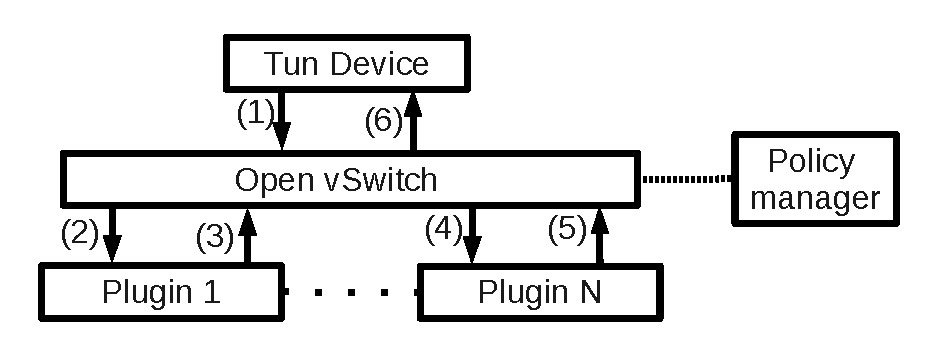
\includegraphics[width=\columnwidth]{figures/packet-monitoring-plugin.pdf}
\end{center}
\vspace{\postfigspace}
\caption{Plugin infrastructure for \platname, which allows traffic to pass through 
a series of middlebox services before being forwarded to the destination. }
\label{fig:packet-monitoring-solution}
\vspace{\postfigspace}
\end{figure}

Once user traffic arrives at the server and is logged, it may be processed by one or more network services.
Figure~\ref{fig:packet-monitoring-solution} shows how 
\platname{} supports a plugin
infrastructure for custom flow processing. Each plugin takes as input a 
network flow and outputs a network flow (potentially empty). 
When a packet is received at the TUN
device, it is sent to a software-defined switch~\cite{Openvswitch} that 
determines the ordered set of plugins that flows will traverse. 
This order is configured by a policy manager, which determines 
the set of plugins that should operate on each flow. After the last 
plugin is traversed, the network flow is sent out through the TUN device 
to the Internet. 

Plugins support a variety of features such as ad blocking, 
analyzing PII leakage or page speed optimization. We 
 use a plugin to enable SSL traffic decryption (described in the previous section) using 
the \platname{} plugin infrastructure. Additionally, we have implemented 
per-connection blocking, malware analysis and DNS-based packet filters. 

\noindent\textbf{Frontend services.} As we describe in \S~\ref{sec:isp-behavior}, 
\meddle supports active measurements. 
Specifically, we inject JavaScript into Web pages to detect if the device's 
access network is modifying Web content in flight, and we use a companion app to 
test detect service differentiation within mobile ISPs. To support these services, we 
run services on \meddle servers that are accessed via untunneled connections. 

\section{Design Evaluation}
\label{subsec:design_deploy}

In section~\ref{sec:user} we described the user experience with \meddle and how its simplicity leads to a low barrier to adoption, while its many services provide incentives for adoption. We also described our system architecture, which allow us to capture {\it all} user-generated traffic and interpose and manipulate it to provide useful services for end users. We now briefly evaluate whether we have achieved all of these goals with {\it low overheads} in terms of network performance, energy usage, and scalability; we then discuss our architecture's strengths and weaknesses more generally. 

\subsection{Overhead Metrics}
\noindent\emph{Network Latency.}
We first test indirection overhead from mobile networks to a \meddle instance. In the 
US with EC2, delays from mobile-network egress points to EC2 nodes are on generally less than 10\,ms. 
For other networks, we will achieve similarly low indirection overhead by placing instances in a cloud/hosting 
provider near subscribers and use DNS redirection (\eg via Amazon's Route 53) to direct clients to nearby instances. 

The other source of network delays is connection establishment time, incurred once per session. We measured 
50 VPN-connection establishment times on both iOS (iPhone 5 / iOS 6.1) and Android (Galaxy Nexus /
Android 4.2), for \wifi{} and cellular connections. We conduct tests in rapid succession to prevent RRC demotion.
The \meddle server was running on a university network. 
For Android (using IKEv2), the maximum establishment time was 0.81 seconds on \wifi{} and 1.59 seconds on cellular. 
For iOS (using IKEv1), the connection takes longer due to the older protocol version: we observe a maximum of 2 seconds on \wifi{} and 2.18 seconds on cellular. 
Because each VPN session supports many flows, the amortized cost of connecting is  small. 
%\tbd{Cite results from latency to home gateways based on DSL results in PAM and IMC.}
%\tbd{Address comments in conext review on latency}

\noindent\emph{Power Consumption.}
Mobile devices expend additional power to establish, maintain and encrypt data for a VPN tunnel. 
To evaluate the impact on battery, we used a power meter to measure the draw from a Galaxy Nexus running Android 4.2. 
We run 10-minute experiments with and without the VPN enabled. 
For each experiment, we used an activity script that included Web and map searches, Facebook interaction, e-mail and video
streaming. 
The VPN leads to a 10\% power overhead. 
For iOS devices, we relied on the battery readings provided by iOS because we cannot attach a power meter directly to the battery.
We again found an approximately 10\% power overhead of using VPNs when we drained a fully charged battery while performing the operations performed during the tests for Android devices.  

%\item 
\noindent\emph{Traffic Volume.}
\meddle relies on IPsec for datagram encryption, thus there is an encapsulation overhead for each tunneled packet. 
To evaluate this overhead, we use 30 days of data from 25 devices that to compare encapsulated and raw packet sizes. 
We observe a maximum encapsulation overhead of 12.8\% (average approximately 10\%). 
For users that have limited data plans and consume most of their quota per month, this can have 
a significant impact. We note that this is partially offset by \meddle services such as content filtering, 
connection blocking and optimizations such as transcoding and compression. 

\noindent\emph{Scalability.} We currently use Amazon EC2 to support users outside of China.\footnote{China 
blocks VPN access to all but domestic destinations; thus, we use a Chinese cloud host (Aliyun) to run  
\meddle in China.} Without exploring opportunities for economies of scale, we estimate that 
it will cost less than a penny (\$0.0084) per user per day. At this cost, we can support up to 
10,000 users with research funds. If \meddle were to become extraordinarily popular, it would 
cost each user approximately a quarter per month to pay their own way. By comparison, 
data plans in the US tend to cost \$30-\$90 per month -- more than two orders of magnitude larger.


\subsection{Discussion}

\mypara{Generalizability} A system for improving visibility and control over Internet traffic from mobile 
devices can be implemented at the endpoints (\eg in the OS), in the network (\eg a hardware middlebox), 
somewhere else in the middle (our approach). \meddle is not intended as a blanket replacement for 
these alternative approaches; rather it allows us to explore the opportunities for improving the state of the 
art in today's mobile systems by making mobile Internet traffic available to researchers. 

In some cases, \meddle is the right location to implement new services that could be costly 
to deploy on devices (prefetching) or impractical to deploy in network (detecting ISP service differentiation). 
In other cases, \meddle provides a practical partial solution to a problem where the complete solution has an impractical 
cost. For example, identifying privacy leaks from mobile devices is reliably addressed using information flow 
analysis~\cite{enck:taintdroid}. However, due to the overheads of this approach it is difficult to deploy to users 
and at scale. \meddle allows us to identify and block unobfuscated PII in network flows from arbitrary devices without requiring 
OS modifications or taint tracking. Regardless of the optimal solution for any single problem, we can use \meddle today to inform the design 
and deployment of future functionality in OSes and for in-network devices. 

\mypara{Limitations} The following technical limitations can impact \meddle's coverage.

%\begin{packeditemize} 
\noindent\emph{Trust.} This paper focuses on a cloud-based \meddle deployment, which requires 
that users trust our system with their network data. We will make our code open source to build this 
trust, however, especially paranoid users may choose not to use our infrastructure at all.

\noindent\emph{At most one VPN tunnel.}
Currently iOS and Android support exactly one VPN connection at a time. 
This allows \meddle to measure traffic over either \wifi or cellular interfaces, but not both at once.
%The vast majority of traffic uses only one of these interfaces, and VPNs can be used to tunnel that traffic.
%\tbd{MPTCP on iOS 7??}

\noindent\emph{Proxy location.} 
When traffic traverses \meddle, destinations will see the \meddle box address, not the device IP, as the source. 
This may impact services  that customize (or block access to) content according to IP address (e.g., in case of localization). 
A solution to this problem is to use a \meddle{} instance with a localized IP address.

\noindent\emph{ISP support.}
Very few ISPs block VPN traffic: there is a disincentive to doing so due to enterprise clients. However, to do so would block access to our \meddle implementation. 

\noindent\emph{IPv6.}
\meddle{} cannot be currently used on networks using IPv6 because IPv6 is not fully supported by mobile devices. 
%Indeed, we observe that though iOS and Android support IPv6 they currently do not support IPv6 traffic through VPN tunnels.
%\end{packeditemize} 


%\noindent\item \textbf{Wi-Fi Gateways powered by Cellular Modems.}


%\subsection{Costs}
%
%\noindent\textbf{Deployment and Running Costs}
%
%\noindent\textbf{Trust Provider}
%
%\subsection{Incentive for Deployment}
%
%\noindent \textbf{Deploy on Home Gateway.}
%This is why we need the single machine constraint. 
%
%\noindent \textbf{Packet Filtering.}
%Custom ad blocks. Protect against data leaks. 
%
%\noindent \textbf{User Interface to Packet Filtering.}
%
%\noindent \textbf{Security from untrusted Wi-Fi APs.}
%
%\subsection{Current Deployment}
%
%\footnote{\meddle is currently in private beta with deployments in the US, France and China. Users sign-up for an IRB approved study through \url{http://meddle.mobi}. We will make the \meddle software publicly available.} 
%
%\subsection{Discussion}




%\noindent \textbf{Modular Architecture for Offloading Activities.}



%%% Local Variables: 
%%% mode: latex
%%% TeX-master: "meddle-main"
%%% End: 
